% Условная компиляция для самостоятельной работы
\ifdefined\mainfile
    % Если это часть основного файла, не добавляем начало и конец документа
\else
    \documentclass[12pt, a4paper]{report}
    \usepackage{/Users/vladbelousov/Desktop/Semestr_4-FP-NSU/Настройка/library}
    \usepackage[utf8]{inputenc} % Подключение поддержки UTF-8
    \begin{document}
\fi

%%-------------------------------%%

\[ \vec{E }  _{\Sigma} = \sum_{m=1} ^{ M_0 } e^{i \omega_0 (t - t_m ) - \gamma (t - t_m ) }\vec{E }  \underbrace{\left( \frac{L}{\gamma_m }  \right)}_{\approx 1 } = e^{ i \omega_0 t - \gamma t } \underbrace{\sum \vec{E }  _0 e^{ i \omega t_m + \gamma t_m }}_{= \vec{E}  _{oo } \text{ постоян. вектор}  }     \]  



Рассмотрим эволюцию поля \( E_{\Sigma }  \) после выключения источника появления новы излучающих атомов. 

\begin{center}
    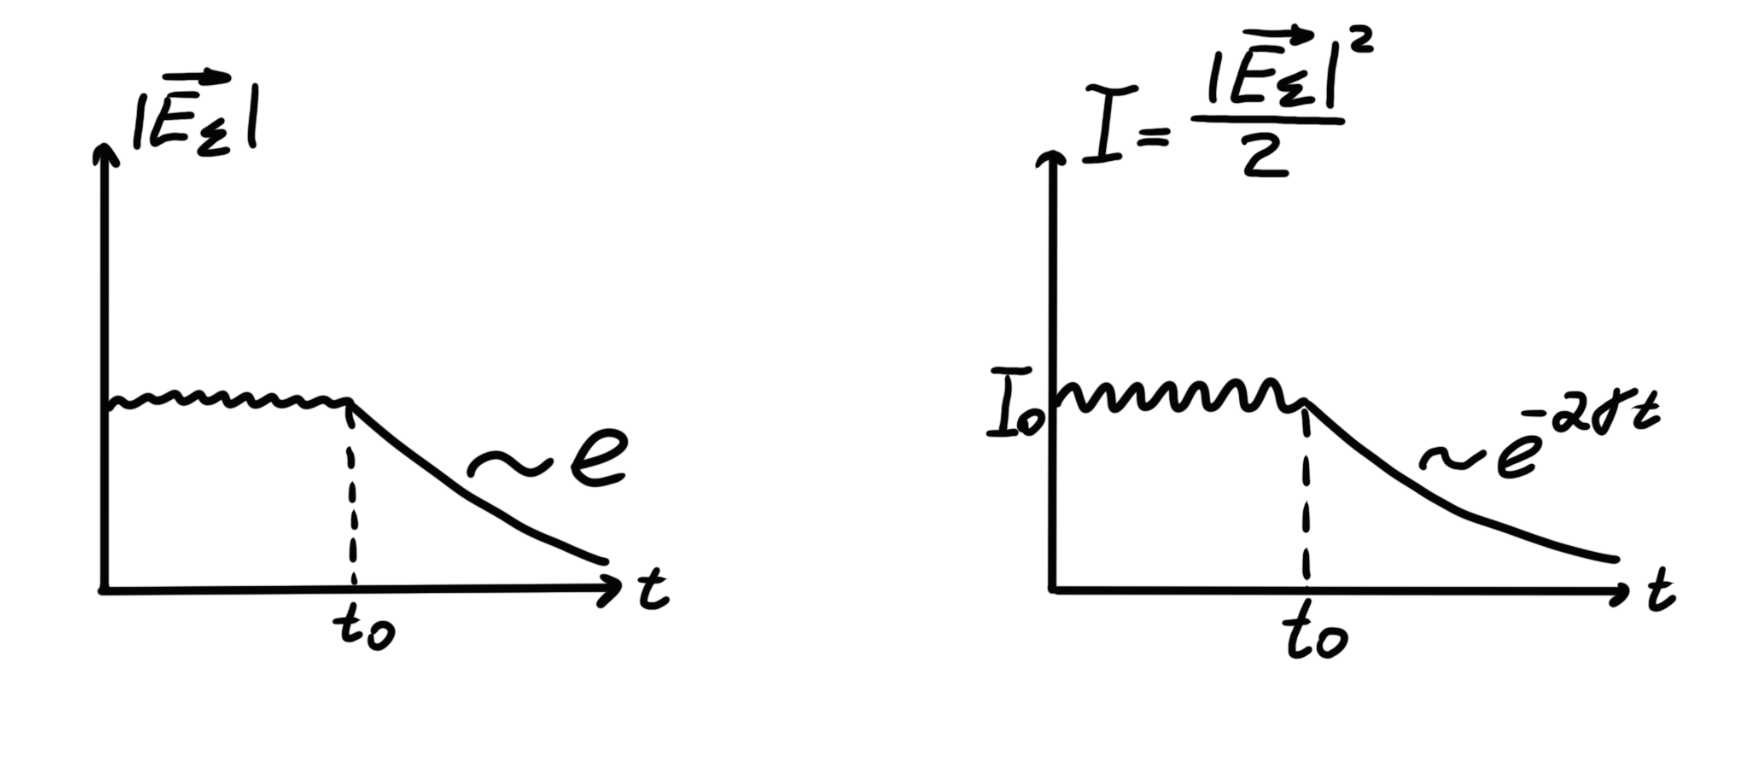
\includegraphics[width=0.5\textwidth]{/Users/vladbelousov/Desktop/Semestr_4-FP-NSU/ЭиО/Лекции_по_дням/image/99.png}
\end{center} 
При \( \displaystyle t > t_0 \quad  I(t ) =I_0 e^{-2 \gamma t } \Rightarrow \frac{dI}{d t }  = - 2 \gamma I(t )  \) 

Так как число членов ряда в сумме \( \displaystyle  \sum_{m =1} ^{M_0}   \) с ростом времени растет, а вклад атомов начавших излучать с самых ранних времен, экспоненциально мал, то введем \( N_{\text{эф} }  \) - число эффективно излучающих атомов: 

\[ I(t) = N_{\text{эф} } \frac{|\vec{E } _0     | ^2 }{2 } \Rightarrow \frac{dN_{\text{эф} } }{dt }  \cdot \frac{ |\vec{E } _0| ^2 }{2 } = - 2 \gamma N_{\text{эф} } \frac{|\vec{E } _0  | ^2 }{2 }  \] 
\[ \frac{d N_{\text{эф} } }{dt } = - 2 \gamma N_{\text{эф} } + p  \] 
, где \( p \) - скорость появления новых излучающих атомов \( \Rightarrow  \)  в стационарном  процессе \(: \displaystyle  \frac{d N_{\text{эф} } }{dt } =0 \Rightarrow p = 2 \gamma \overline{N}_{\text{эф} }    \) 

%img

\[ \vec{E }  _0 = E_{0x }  \vec{e}_x + E_{0 y }  \vec{e }  _y , \quad  E_{0 x }  \text{ и } E_{0 y}  \in \mathbb{C}    \] 

Так как \( \displaystyle  I_{12} = \mathrm{Re }  (\vec{E }  _1 (\vec{r } ), \vec{E }  _2^* (\vec{r } )) = 0 , \text{ при } \vec{E }_1 \perp \vec{E } _2   \), то \( I_x \text{  и } I_y  \)  не интерферируют и могут быть вычислены отдельно: 

\[ I = I_x + I_y = <(\mathrm{Re}  \vec{E }  _{\Sigma x } (t )  ) ^2> + <(\mathrm{Re}  \vec{E }  _{\Sigma y } (t )  ) ^2 > = \] 
\[\kern-1cm =\bigg< \left( \sum_{m=1} |E_{0x} | \cos [\omega_0 (t - t_m ) - \varphi_x]e^{ - \gamma (t -t_n )},  \sum_{n=1} |E_{0x} | \cos [\omega_0 (t - t_n) - \varphi_x]e^{ - \gamma (t -t_n )}\right)\bigg> +<\mathrm{Re }  \vec{E } _{\Sigma y}  >=\] 

\[ I_x = \sum_{n =m } |E_{0x}  | ^2 <\cos  ^2 (\omega_0 (t -t_m ) - \varphi_x )> e^{-2 \gamma (t -t_m )} +   \] 
\[ + \bigg< \sum_{n}\sum_{m} \frac{ |E_{0x } | ^2 }{2 }\left\{ \cos (\omega_0 (2t - t_m -t_n ) - 2 \varphi_x) + \cos \omega_0 (t_m - t_n) \right\} e^{-\gamma (2t - t_m - t_n)}\bigg> \] 
, где во втором членом \(\cos \omega_0 (t_m - t_n)   \) с ростом числа атомов растет \( \sim \sqrt{N_{\text{эф} } } \).

\[ \sum_{m =1}^{\infty  }e^{- 2 \gamma (t - t_m )} \to  \int_{- \infty  }^{t } e^{-2 \gamma (t - t' ) }  \underbrace{p dt '}_{dm } = p (- 1 ) \int_{\infty }^{0} e^{- 2\gamma t''     } dt '' = \frac{p }{2\gamma } = \overline{N }_{\text{эф} }         \] 

\[ I = I_x + I_y     = \frac{|E_{ox }  | ^2 }{2}\overline{N }_{\text{эф} } +\frac{|E_{oy }  | ^2 }{2} \overline{N }_{\text{эф} } = \frac{|E_{o }  | ^2 }{2} \overline{N }_{\text{эф} } \] 

\[ E_{\Sigma x } (t ) = \varepsilon_x(t ) e^{ - i \omega_0 t }   \] 
, где \( \varepsilon(t ) \) - амплитуда \( \in \mathbb{C} \).

\[ <(\mathrm{Re }  E_{\Sigma x }      ) ^2 > = |\varepsilon_{x} (t)|<\cos  ^2 (\omega_0 t - \mathrm{arg }  \varepsilon _x (t ) )> = \frac{ <|\varepsilon_x (t)|>}{2 } = \frac{|E_{0x} | ^2 }{2} \overline{N } _{\text{ эф} }   \] 
\[ <|\varepsilon_x |> = \sqrt{N_{\text{эф} } } |E_{0x } | , \quad  \frac{ \Delta |\varepsilon_{x} |}{|\varepsilon_x|} \approx \frac{|E_{0x} |}{\sqrt{N_{\text{эф} } }|E_{0x} |}  \sim \frac{1}{\sqrt{N_{\text{эф} } }}  \] 

\begin{center}
    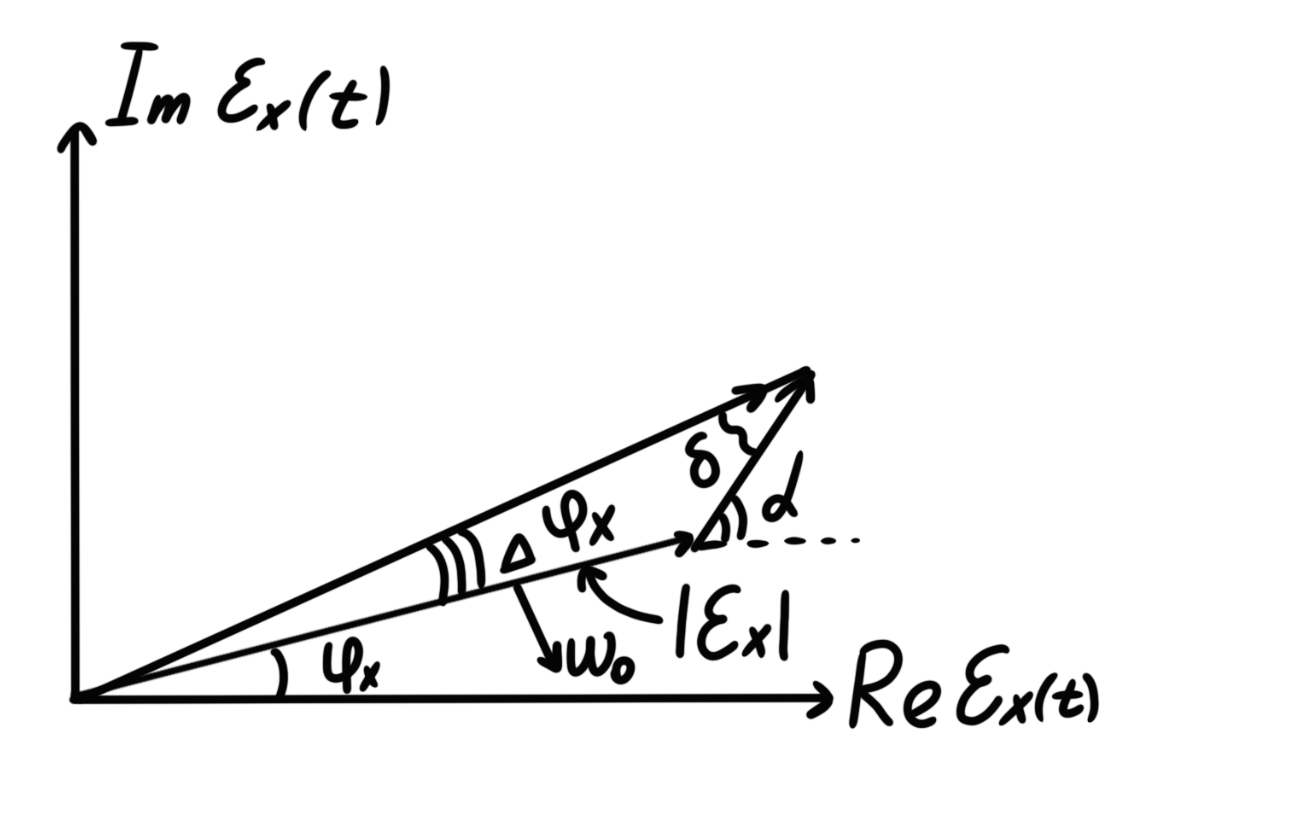
\includegraphics[width=0.5\textwidth]{/Users/vladbelousov/Desktop/Semestr_4-FP-NSU/ЭиО/Лекции_по_дням/image/100.png}
\end{center} 
\[ E_{0x}, \text{ }  \varepsilon_x (t ) \in \mathbb{C}  , \text{ } \alpha  = \mathrm{arg }  E_{0x}    \] 

В момент времени \( t_m = t_{m_0} + \frac{ r_m }{c}   \) начал излучать m-ый атом.

\[ \frac{\sin (\delta \varphi_x ) }{|E_{0x} |} =\frac{\sin \delta}{|\varepsilon_x(t)|}, \text{ т.к } \delta \varphi_x \le 1 \Rightarrow \delta + \pi - (\alpha - \varphi_x ) \approx \pi    \] 
\[ \delta \varphi_x = \frac{ |E_{0x} |}{|\varepsilon_x(t)|} \sin (\alpha - \varphi_x ) = \frac{|E_{ox } |}{|\varepsilon_x(t     )|} \mathrm{ sin }    (\alpha - \omega_0 t_m - \underbrace{\mathrm{arg } \varepsilon_{x } (t )}_{\approx \mathrm{const}  }  )   \] 

\[ <\delta \varphi_x > = 0 , \quad  <\delta \varphi _ x ^2 > = \frac{|E_{0x } | ^2 }{|\varepsilon_x (t )| ^2 } \frac{1}{2 } = \frac{1}{2 N_{\text{эф} } }    \] 

Коэффициент диффузии по \( \varphi_x \) (аналогично броуновскому движению) вычисляется так: 

\[ \frac{<\delta \varphi_ x  ^2 >}{\Delta t } = \frac{<\delta \varphi _x ^2 >}{\frac{1 }{p } } = \frac{p}{2N_{\text{эф} } } =   \gamma  \] 
, где \( \Delta t \) - характерный промежуток времени между появлением новых атомов. Пусть \( \displaystyle <\delta \varphi ^2 > = 1 \Rightarrow \Delta t_0 = \frac{1}{\gamma}  \) 

\begin{center}
    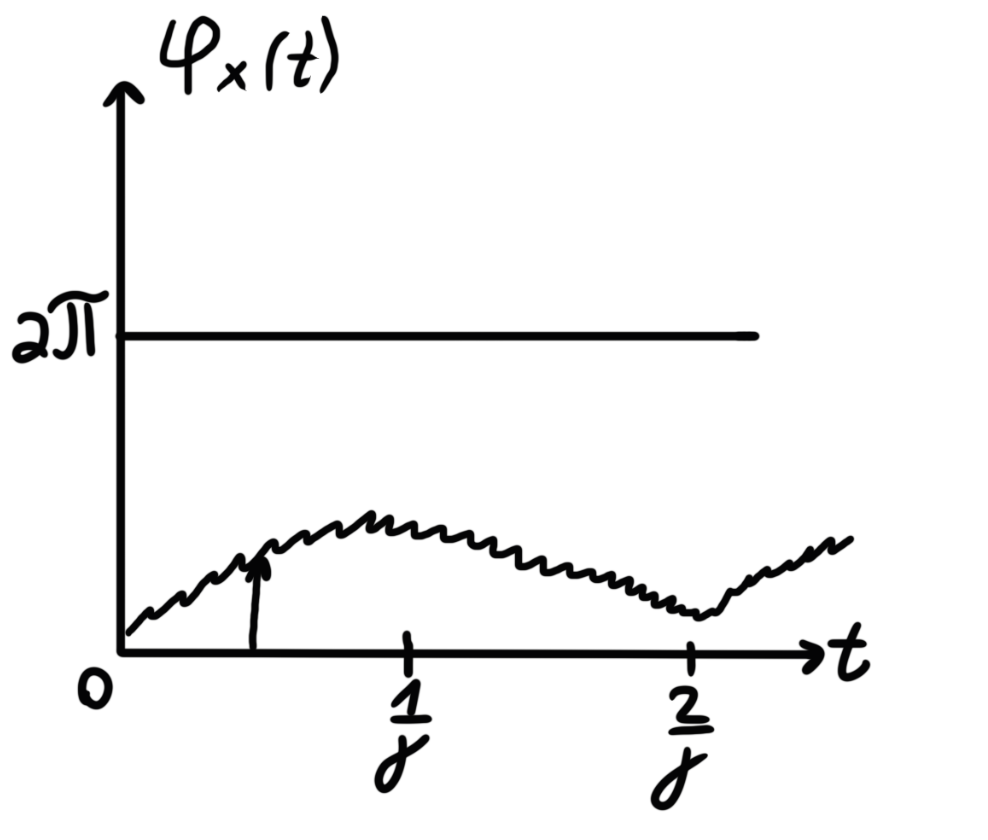
\includegraphics[width=0.4\textwidth]{/Users/vladbelousov/Desktop/Semestr_4-FP-NSU/ЭиО/Лекции_по_дням/image/101.png}
\end{center} 

Изменение \( \delta \varphi_x  \) на  \( \Delta t < \Delta t_0 = \frac{1}{\gamma }   \) мало (фаза почти постоянная), а на \( \Delta t  > \Delta t_0  \) фаза \( \varphi _x (t )  \) - случайная величина \( [0, 2\pi ] \)  

Вывод: в стационарном случайном процессе излучения скопления атомов амплитуда суммарной волны почти постоянная  \( \left( \text{флуктуации }  \displaystyle  \frac{\Delta \varepsilon }{\varepsilon }\sim \frac{1}{\sqrt{N_{\text{эф} } }} \right)   \), а фаза этой волн почти постоянна на промежутках \( \displaystyle  \Delta t < \frac{1}{\gamma }  \) и случайно меняющаяся величина на \( \displaystyle  \Delta t > \frac{1}{\gamma }  \). 

\begin{center}
    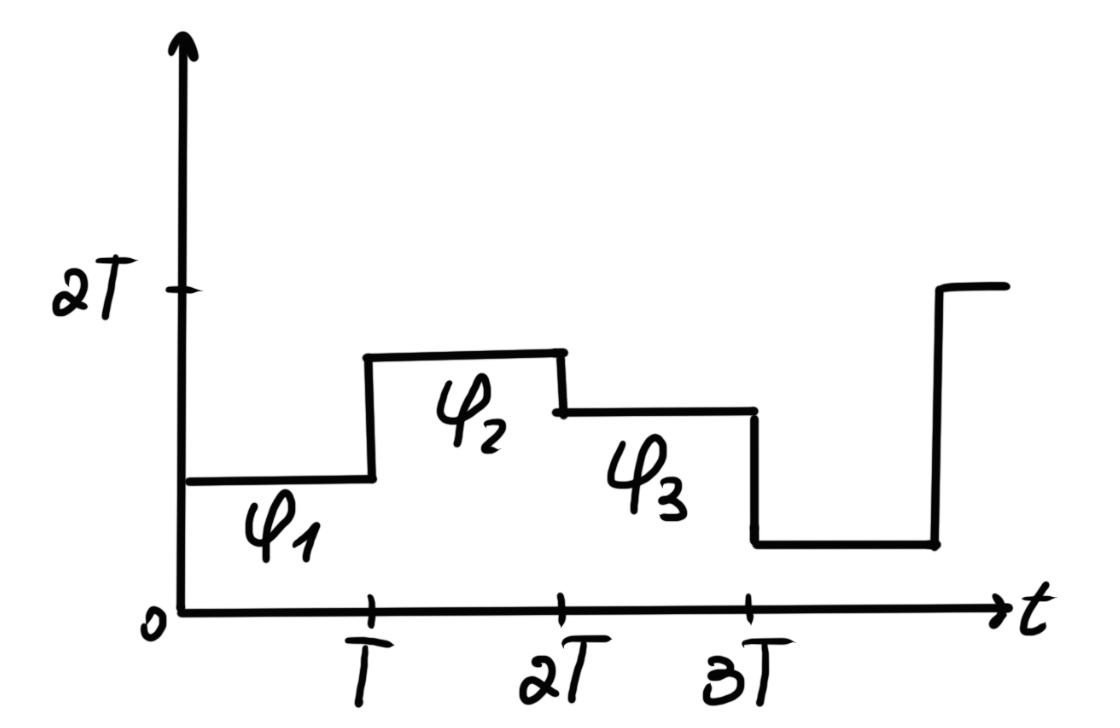
\includegraphics[width=0.4\textwidth]{/Users/vladbelousov/Desktop/Semestr_4-FP-NSU/ЭиО/Лекции_по_дням/image/102.png}
\end{center} 

Приближенная модель такого поля  \( \varepsilon _x = \mathrm{const }   \), а \( \varphi _ x (t )  \)   случайная величина в \( [ 0 ,2 \pi] \).

Вычислим спектр суммарного поля: 

\[ \vec{E } _{\Sigma } (t ) = \sum   \vec{E }  _ 0 e^{ - i \omega_0 (t -t_m )- \gamma(t- t_m)}   \] 

\[ \hat{\vec{E } } _{\Sigma } (t ) = \sum_{m }\hat{\vec{E }}   _ a(\omega ) e^{i \omega t_m}     \] 

Спектральная плотность энергии: \(  \displaystyle  |\vec{E } _{\Sigma } ( \omega ) | ^2 = \left( \sum_{m }\hat{\vec{E } }_a (\omega ) e^{i \omega t_m } , \sum_{n}\hat{\vec{E } }_a ^{*} (\omega ) e^{-i \omega t_n }   \right) = \) 
\[ |\vec{E } _a ( \omega)    | ^2 \left\{  \sum_{n =m  =1 } ^{N_{\text{эф} } } 1 \sum  ^{N_{\text{эф} }  } _{n }  \sum_{m} ^{N_{\text{эф} } } e^{ i \omega (t_m - t_n)}   \right\}  \Rightarrow |\vec{E }  _{\Sigma } ( \omega ) | ^2  = |\hat{ \vec{E } } _a ( \omega ) | ^2 N_{\text{эф} }\] 

\begin{center}
    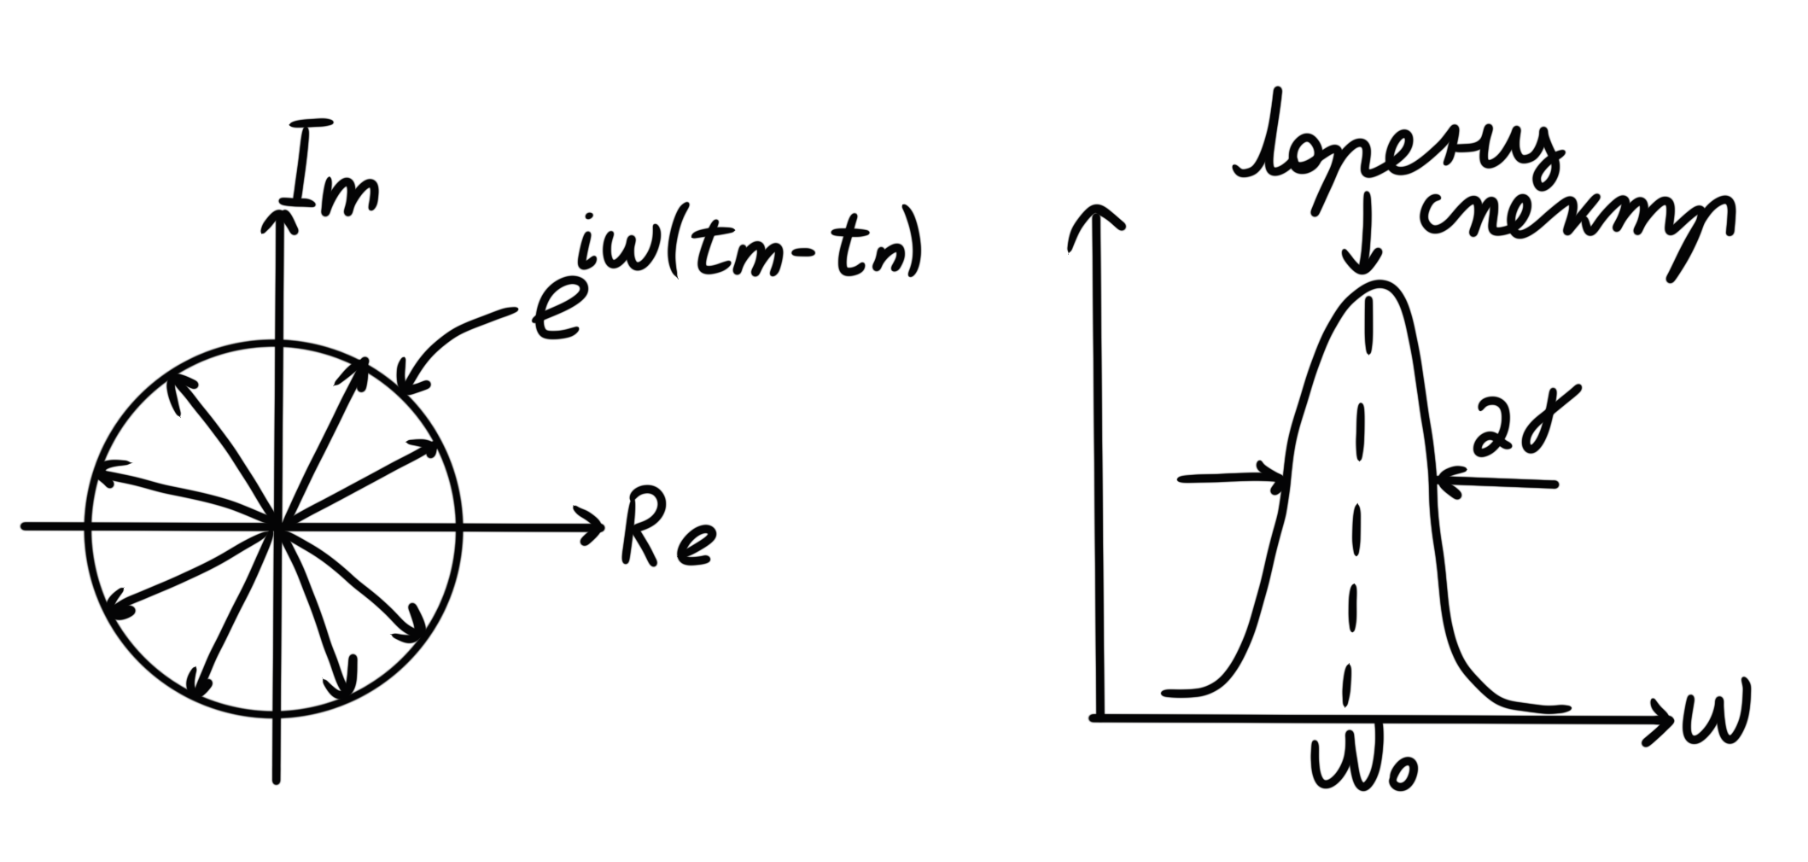
\includegraphics[width=0.5\textwidth]{/Users/vladbelousov/Desktop/Semestr_4-FP-NSU/ЭиО/Лекции_по_дням/image/103.png}
\end{center} 

\textbf{Опыт Юнга: } 

\begin{center}
    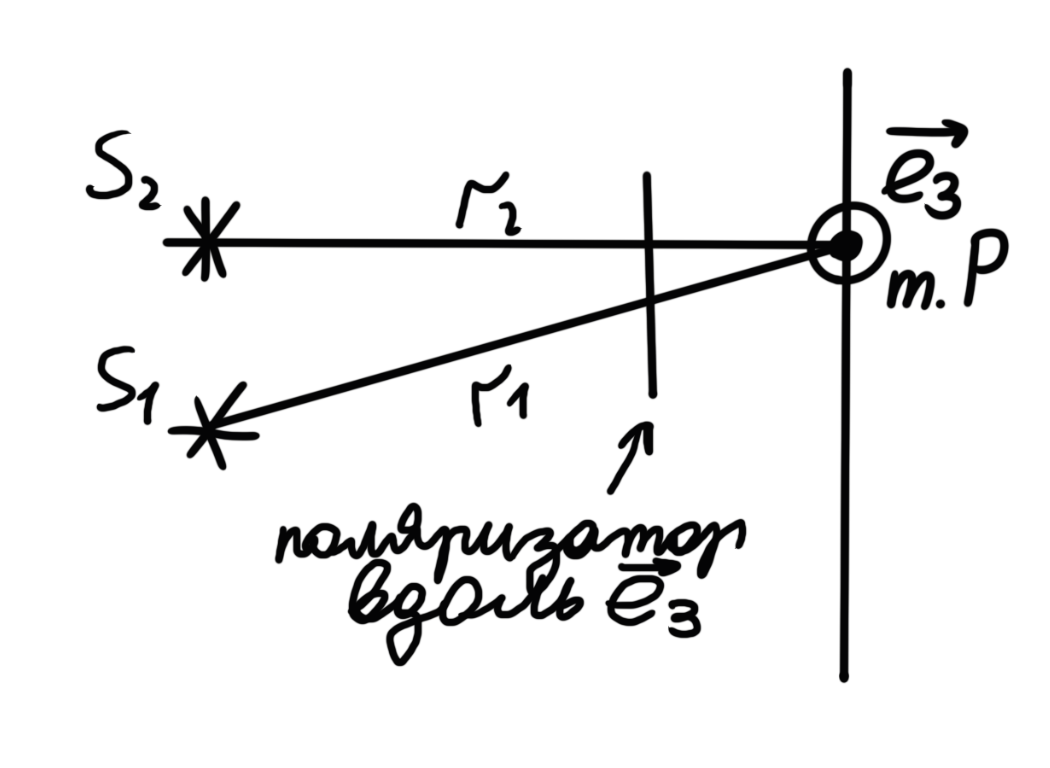
\includegraphics[width=0.4\textwidth]{/Users/vladbelousov/Desktop/Semestr_4-FP-NSU/ЭиО/Лекции_по_дням/image/104.png}
\end{center} 

\[ \vec{E }  _{\Sigma 1 } = \vec{E }  _{01 }  \frac{L}{r_1 } e^{ i k r_1 - i \omega_0 t + i \varphi_1 (t )}    \] 
\[ \vec{E } _{\Sigma_2 } = \vec{E }  _{02 }  \frac{L}{r_2 }e^{i k r_2 - i \omega_0 t + i \varphi_2 (t)}    \] 

\[ I_{12} =  <\mathrm{Re }  (E_{ \Sigma_1 }, E_{ \Sigma_2 }^* )   > = |\vec{E }  _{01 } | |\vec{E }_{02} |\frac{L ^2 }{r_1 r_2} <\cos (k(r_1 -r_2 )+ \varphi_1 (t ) - \varphi_2 (t))>   \] 

Если временное разрешение прибора \( \tau_0< \)время  изменения фаз \( \varphi_1 \text{ и  } \varphi_2  \left( \sim \displaystyle \frac{1}{\gamma}  \right) \), то интерференционная картина видна и поля когерентные. 

Если \( \tau_0 > \displaystyle \frac{1}{\gamma}  \), то \( <\cos ()>  = 0 \Rightarrow \) поля некогерентные.

%%-------------------------------%%

% Закрытие документа, если файл компилируется отдельно
\ifdefined\mainfile
    % Если это основной файл, не нужно заканчивать документ
\else
    \end{document}
\fi

